\chapter{SER Simulations and Results}\label{ch-ser_sim}
This section discusses the experimental procedure of using CyTex to generate RGB images and the construction of a DCNN model to extract features and classify the dominant emotion of each CyTex image passed through the model. It is of importance to note that machine learning results can often be hardware dependent and difficult to reproduce, even under the same experimental conditions. The Initial simulation results and improved results are both discussed. This is to inform the reader of the dependency on hardware related to performance. It also highlights the nature of machine learning problems, which often require significant tuning and reconstruction to achieve more desirable results. Through this chapter, the engineering design process should also be acknowledged; making informed decisions and balancing trade-offs to improve system performance. 

% SECTION:
% ================================================
\section{Experimental Environment}
All programming of this project took place in Python. The Integrated Development Environment (IDE) utilised was PyCharm on certain local machines and VSCode in other instances. GitHub was used for centralized version control of the project. The GitHub repository for this project can be accessed through the following reference \cite{Blake_ELEC4840B-Repo}. Further information regarding the structure and functionality of the code can be found in the \textit{readme.md} file of the aforementioned repository.\\ \\
The deep learning component of this thesis was carried out using PyTorch and it's associated deep learning deep learning frameworks \cite{PyTorch_Ketkar_2017}. The office spaces and computers in \textit{ES-219} and \textit{ES-115A} were utilised for preliminary code building and DCNN simulation, respectively. Sufficiently advanced contemporary equipment is required to complete deep learning simulations in a reasonable amount of time. Specifically, deep learning simulations should be conducted on platforms with appropriate graphics cards to enable parallel processing. This hardware not only effects the time of simulations, but also the quality and accuracy of results. IThe hardware specifications of the work station present in \textit{ES-115A} include an Intel Core i7-7800X CPU at 3.5GHz, 2 threads per core and 6 cores per socket. The memory is rated as 32 GB DDR4 memory. Finally, a CUDA enabled graphics card was utilised for deep learning simulation. The graphics card utilised was an NVIDIA GeForce GTX 1080 Ti with a 33MHz clock.

% SECTION:
% ================================================
\section{Generating CyTex Images}
The generation of CyTex images for all databases detailed in this thesis followed the structure highlighted in chapter \ref{ch-theory}, figure \ref{cytexFlowchart}. However, this section gives further specificity with respect to the programming and construction of the process. Choices for important parameters are also discussed.
\subsection{Loading and Resampling}
Initially each of the \textbf{.wav} files are loaded using the glob python library which allows for UNIX based string specifications. After all file names are appended to a list, each audio file is loaded using the librosa python package (version 0.8.1) \cite{brian_mcfee_2021_4782663}. Librosa is also used to resample the loaded signal at a new sampling rate of $16kHz$. This is a standard sampling rate for speech signals as all most speech is generated at frequencies below $8kHz$. By accounting for the Nyquist criterion, we sample at twice this rate.\\ \\
\subsection{Frame Division and Overlap}
The resampled audio signals are then divided into smaller frames in two separate steps. Firstly, a signal will be split into relatively larger frames of $16000$ samples. Due to our sampling rate, this is equivalent to one second in the time domain. Each of these one second frames constitutes some portion of the original emotional audio file. It is important to note that a CyTex image is generated for each one second frame, and not for every full audio file. This naturally inflates the dataset as more CyTex images are generated than \textbf{.wav} files existed in a given dataset. As size is often largely limited in SER datasets, this helps in reducing the overfitting of a model trained on CyTex data. An overlap parameter can be adjusted to allow the inclusion of data between neighbouring one second frames. This parameter is labelled \textit{n\_step} and the overlap is given by equation \ref{overlap_eq}.
\begin{align} \label{overlap_eq}
    overlap &= 100 \times \dfrac{n_{step}}{f_s} (\%) \\
            &= 100 \times \dfrac{n_{step}}{16000} (\%) \nonumber
\end{align}
This overlap parameter is included to allow for modelling of the continuous nature of a speech signal. This parameter was marginally tuned, however, it was later determined no overlapping of the signals marginally improved the accuracy results.\\ \\
After this the approximately one second frames were further decomposed into 100 sub-frames. This gave each frame an approximate width of $10ms$, chosen due to the stationary approximation of speech over this interval.

\subsection{Pitch and Magnitude Extraction}
The fundamental frequency (pitch), as previously noted, was extracted using the librosa piptrack method. The index of the largest magnitude was found for each sub-frame, as well as the corresponding pitch. During pitch extraction minimum and maximum frequency thresholds are provided to the piptrack method. These parameters can impact the quality of the generated CyTex image quite largely. A minimum threshold of $40Hz$ was chosen to include lower frequencies of human speech and an upper threshold of $400Hz$ was arbitrarily chosen. If these parameters do not include the window of frequency of typical human speech, no emotional classification will be able to be made. Different windows are also able to be specified to the piptrack method, however, this functionality was not explored.

\subsection{Image Dimensions and Processing}
The number of vertical rows present in the CyTex image is detailed in equation \ref{vert_rows_eqn}. The horizontal width of figures was constant across all images generated and found via equation \ref{max_width_cytex}. Upon constructing the image dimensions, the image values were converted from a list to a numpy array and normalized. A form of increased contrast was applied to the values via raising all pixel values of the image to the third power. Mathematically, this increases the larger valued samples and decreases the smaller valued samples with respect to each other. As the output image is an RGB image, three channels of information are available to be encoded. The first channel was encoded with pixel intensity. The remaining channels were encoded using the vertical and horizontal gradients. However, other strategies like the Laplace transform or Gaussian filtering may also be applied. Gradients were chosen as they have the most analogical fitting to the speech domain. One can interpret a derivative related to pitch as an increasing or descending pitch with respect to time.

\subsection{CyTex Image Output}
Upon encoding the three channels of the numpy array, the \textit{Image.fromarray()} method was used to create an output image of RGB type. The size of each image was set to a 400 pixel squared grid. Finally, each image had its corresponding input filename read to determine the associated emotion of the sample. Images were saved into files of each emotional class type (varying depending on which dataset was in use). 

% SECTION:
% ================================================
\section{DCNN Model Architecture}
This section details the selection and additions made to a pre-existing powerful DCNN model, leveraging the power of transfer learning. Utilising transfer learning is the key advantage gained through solving SER problems in the image domain. Many powerful pre-built models already exist in the image domain, (many trained on the ImageNet dataset \cite{deng2009imagenet}).

\subsection{Base Model - ResNet Variants}
One of the most difficult processes in training a deep learning model is finding suitable initialisations for the weights of the system. Initial weights largely influence a machine's ability to learn. Thus, they are vital for notable accuracy on any task. As DCNN's create complex features hierarchically from simpler ones, these initial weights also form the basis on which all features are created.\\ \\
It is not feasible, nor possible, in this case  to attain great initial weights directly. This is because the datasets for SER are much smaller than image classification datasets like ImageNet \cite{deng2009imagenet}. Created for the advancement of computer vision and object classification, ImageNet boasts 3.2 million images. Within this set there are 12 subtrees, which are essentially broad classes of object. For each of these subtrees there exists 5247 synonym sets. A synonym set is broadly defined by the documentation as "a meaningful concept..., possibly described by multiple words or word phrases". Each of the images present in this dataset are also annotated by humans, ensuring no misclassification in its construction.\\ \\
If a model has been trained on a large image dataset like ImageNet, it can be assured that it possesses the ability to extract features from a wide variety of images. Referring to comments made on the initialisation of weights prior, ImageNet trained models can proficiently extract features from images like CyTex. It is through modifying these models and retraining portions of the networks that we can then select which extracted features are appropriate for classification of CyTex images. \\ \\
A number of readily available models are accessible via the \textit{torchvision.models} subpackage. each of these models comes with their associated pre-trained weights. Common image classification models used via transfer learning include VGG variants, ResNet variants and ConvNeXt. However, due to the scalability and reduced complexity of ResNet models, as well as higher accuracy on similar problems in previous studies \cite{CyTexRef}, the ResNet family was chosen. The ResNet class of models was designed to reduce the complexity of deeper models and eliminate the drawbacks associated with increasing model depth. The key design concept of ResNet was \textit{"reformulating layers as learning residual functions with reference to the layer inputs, instead of learning unreferenced functions"} \cite{he2015deep}. This reformulation involves recasting the desired underlying mapping of $\mathcal{H(\mathbf{x})}$ as $\mathcal{F(\mathbf{x})} \coloneqq \mathcal{H(\mathbf{x})} - \mathbf{x}$. Results of this method have yielded extremely high accuracy, even taking first place at the 2015 ImageNet Large Scale Visual Recognition Challenge (ILSVRC). Various depths of models are available including 18, 34, 50, 101 and 152 layer models.

\subsection{Retraining \& Improving Generalization}
The deeper ResNet models like the 101 and 152 layer variants required too much memory to operate reasonably on the experimental environment. While the batch size could have been decreased to accommodate this, the training process would have taken much longer and rapid pilot testing would not be possible. Resulting in much slower pilot testing results. The complexity of these deeper models would likely result in higher classification accuracy, however, it is hypothesised that this would not be to a dramatic extent.\\ \\
The first two layers of weights of the ResNet model were "frozen". Meaning they were fixed to their original values during the training phase of model fine-tuning. This design consideration was to allow a sufficient initialisation while still providing enough weights to retrain to offer specificity in the classification of CyTex images. Since the structure and composition of CyTex images differ significantly to many images present in ImageNet (the basis of training for ResNet) significant adaptation to later weights was required.\\ \\
\subsubsection{Model Output Layers}
As the original ResNet structure is designed to classify data over 1000 different classes, the output of the model had to be altered. Additions to the output of the original model are listed below. Additional layers introduced to the output of the ResNet model were added with the primary intention of improving model generalisation and specifying the classification to CyTex images.
\begin{itemize}
    \item A dropout layer was added for regularization, enhancing the generalization of the model.
    \itemsep0em
    \item A flatten operation was then used, converting the input tensor into a one-dimensional tensor, to allow input into the subsequent linear fully connected layer.
    \itemsep0em
    \item This linear layer mapped the tensors at the output of the ResNet model (with number of features depending on the model utilised) to a tensor with 4096 features. This layer provides additional learning capacity, further fine-tuning the model to the CyTex data.
    \item A 1-dimensional batch normalization was applied to improve training stability, rate of convergence and additional improve generalizability (although much less so than dropout).
    \itemsep0em
    \item Another dropout layer was used, further reducing the potential for overfitting of the model.
    \itemsep0em
    \item Another linear layer was introduced mapping the aforementioned 4096 features to a smaller set of 1024 features.
    \itemsep0em
    \item A second one-dimensional batch normalization was applied to the data passing through the model.
    \itemsep0em
    \item In order to output predictions over the range of classes of the given dataset, a final linear layer was introduced. This mapped the remaining number of features to the number of classes pertaining to the desired SER dataset.
    \itemsep0em
    \item The final layer used was a softmax function which returned a normalized probability distribution over each of possible output emotional classes. By taking the maximum of the output vector, one yields the class with the highest prediction probability.
\end{itemize}


% \subsection{Model Overfitting - Proof of Concept}
% POTENTIALLY NOT NECESSARY... ONLY INCLUDE AFTER ALL ELSE
% If the model can overfit, then it is working successfully. Can talk about data leakage problems encountered to prove model functionality.

% SECTION:
% ================================================
\section{EMODB Simulations}
This section details the experimentation process used for the EMODB dataset used to select an appropriate model and model parameters. Both successful results and subpar results are discussed in the pilot testing portion to inform the reader of the modifications made throughout the experiment. Design decisions are discussed with reference to the results obtained. These results, for the most part, also informed the design decisions made during RAVDESS testing. This was because the datasets used for training are quite similar in nature, especially when converted to the image domain via CyTex transform.\\ \\
CyTex images were generated using the parameters and techniques specified earlier in this chapter. A random sample of the generated images is provided in figure \ref{emodb_cytex_imgs}, with corresponding class labels. The classes are annotated in the German letter abbreviation format. For translation to English, table \ref{EMODB_emo_table} should be consulted. Please note that each of the images in figure \ref{emodb_cytex_imgs} have not had any form of data augmentation applied to them. This sample, along with the remaining dataset, formed the input for the image classification model.
\begin{figure}[ht]
        \centering
        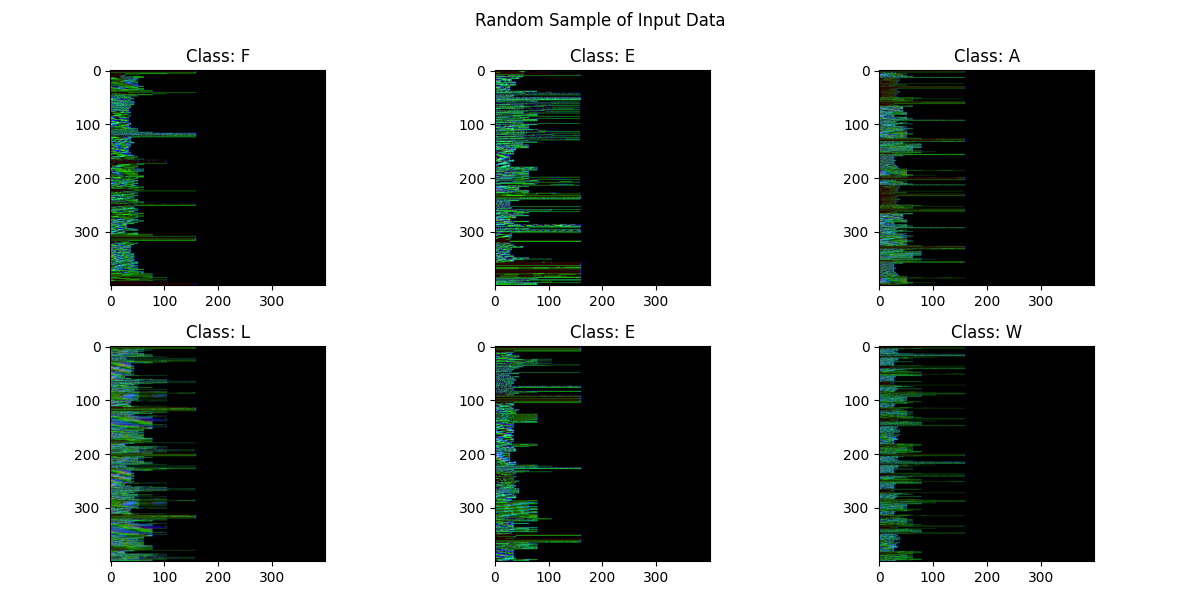
\includegraphics[scale = 0.4]{images_results/CyTex_T1-Initial_Pics/Random Input Sample.png}
        \caption{EMODB - Random CyTex Sample}
        \label{emodb_cytex_imgs}
\end{figure}

\subsection{Pilot Testing and Alterations}
Initially a series of pilot tests were conducted to gauge suitable hyper parameters fro use in the deep learning model. A single simulation was run for varying sets of parameters and the validation accuracy was used to determine the performance of the model. It must be noted that, due to the small size of the EMODB dataset, overtraining is difficult to avoid. By training for a smaller number of epochs with fast convergence, this was marginally mitigated. While pilot tests were conducted on the EMODB dataset, due to the similarity of CyTex images that would be generated for the RAVDESS dataset, the same final hyper parameters were used in that case as well. For each of these trials the EMODB database was randomly split into a train and test set. $80\%$ of the data was grouped into the training set and the remainder into the test set. The random splitting was performed while preserving the balance of classes in both of the data subsets.

\subsubsection{Pilot Test 1:}
For the first pilot test a relatively larger learning rate was employed to allow the model to search rapidly. The ADAM optimization method was used due to its faster convergence than other methods like SGD. It also offers better performance for smaller datasets that can be more prone to noise. A cross entropy loss criterion was also used, which is typical in many image processing tasks. No learning rate scheduler was used as the search habits of this particular learning rate were to be investigated prior to fine tuning. The full list of notable parameters are detailed below.
\begin{itemize}
    \item base model = ResNet50
    \itemsep0em
    \item epochs = 20
    \itemsep0em
    \item mini batch size = 32
    \itemsep0em
    \item $lr = 1e^{-3}$
    \itemsep0em
    \item ADAM weight decay parameter ($\lambda$) = $1e^{-5}$
    \itemsep0em
    \item CyTex overlap = $50\%$
    \itemsep0em
    \item data augmentation (training) = random horizontal flipping and normalization
    \itemsep0em
\end{itemize}
As can be observed in figure \ref{Pilot1_fig}, the convergence for this particular learning rate is far too unstable. That is to say that between epochs the test/validation accuracy is prone to massive fluctuations. This is somewhat unavoidable for smaller non-ideal datasets, however, can be reduced considerably. The best test accuracy achieved in this case was $56\%$. As the training accuracy also seemed to reach a relative ceiling at around $60\%$, it seemed as though the model was having trouble generalizing. By increasing the weight decay parameter ($\lambda$) regularization is also increased. This reduces how large weights can become, in turn reducing model complexity. This parameter was to be modified in future trials.
\begin{figure}[ht]
        \centering
        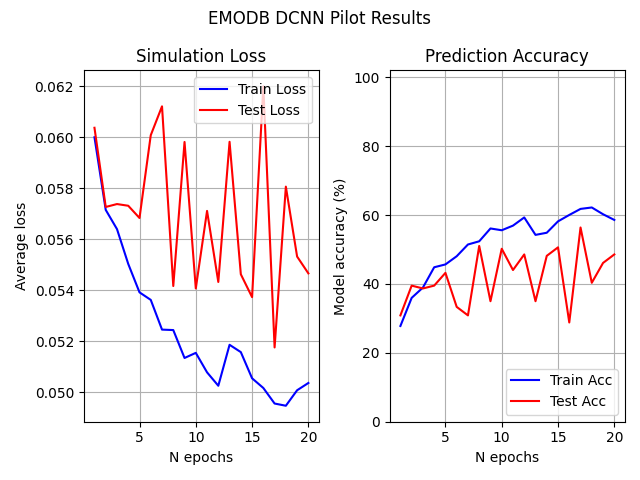
\includegraphics[scale = 0.6]{images_results/EMODB_PilotTests/EMODB_PilotResults_30-05__15-48.png}
        \caption{EMODB - Pilot Test 1}
        \label{Pilot1_fig}
\end{figure}

\subsubsection{Pilot Test 2:}
In the second pilot trial the learning rate was decreased to provide more stable convergence (at the cost of speed). The weight decay was increased to attempt to improve model generalization, reducing large weights present in the model. The number of epochs was also reduced to allow for more rapid pilot testing. While it appears that the model can be trained for longer as the accuracy is still  increasing, this training period is sufficient for parameter comparison and tuning. All parameters not listed below for this trial and future trials can be assumed to be held constant from the previous trial(s). 
\begin{itemize}
    \item epochs = 10
    \itemsep0em
    \item $lr = 1e^{-4}$
    \itemsep0em
    \item $\lambda$ = $1e^{-4}$
    \itemsep0em
\end{itemize}
In this case the convergence was actually faster and more stable. This suggests that the previous learning rate was too large and the model was potentially 'stepping over' local minima and initially missing the ideal solution. The training accuracy was much improved in this trial, informing us that the model is learning more details about the training set. With this more informed model, the test accuracy also slightly improved, reaching a height of $59\%$. It is still apparent that, due to the large difference in training accuracy and test accuracy, the model generalization could be improved. However, the small size of this dataset bring about a fundamental limitation to generalization. 
\begin{figure}[ht]
        \centering
        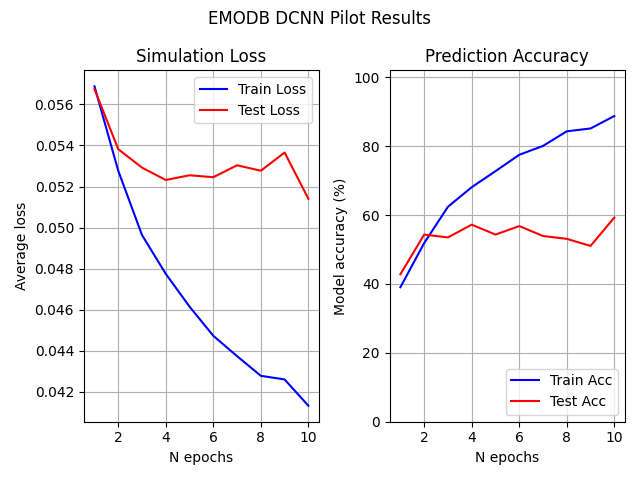
\includegraphics[scale = 0.6]{images_results/EMODB_PilotTests/EMODB_PilotResults_30-05__15-59.png}
        \caption{EMODB - Pilot Test 2}
        \label{Pilot2_fig}
\end{figure}

\subsubsection{Pilot Test 5:}
Pilots 3 and 4 marginally improved accuracy via increasing the learning rate, and hence the search capacity. The number of epochs was also slightly increased. However, due to the minor changes to both parameters and results they are not detailed. Both of these approaches exhibited unstable convergence, as one would expect for a larger learning rate. The fifth pilot test sought to build upon previous trials by attempting to massively improve generalization. The weight decay was increased by a large rate and a number of additional data transformations were applied to the training set, listed subsequently.
\begin{itemize}
    \item epochs = 15
    \itemsep0em
    \item $lr = 1e^{-2}$
    \itemsep0em
    \item $\lambda$ = $1e^{-1}$
    \itemsep0em
    \item data augmentation (training) = random vertical flipping, random rotation, random resized cropping, random horizontal flipping and normalization
    \itemsep0em
\end{itemize}
The results of this test are depicted in figure \ref{Pilot5_fig} and highlight a much more gradual increase in training and test accuracy. A similar scenario was later tested over a larger number of epochs. One may note the much smaller gap between train and test statistics, however, both accuracies are poor. This suggest that the many data augmentation applied, along with increased weight decay, do not allow the model to sufficiently learn the training data. The largest test accuracy obtained over this training interval as $42\%$.
\begin{figure}[ht]
        \centering
        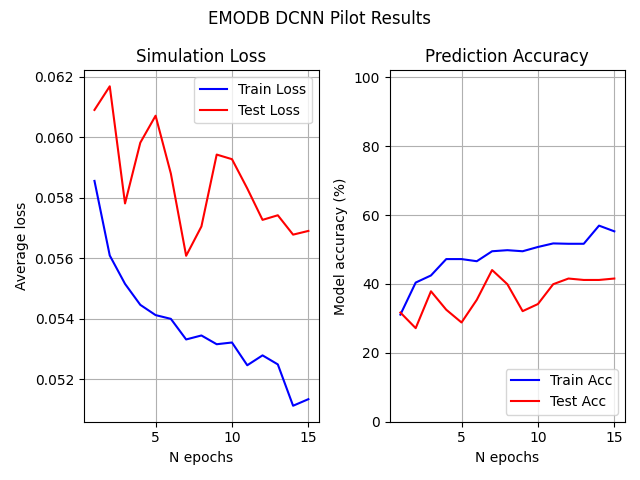
\includegraphics[scale = 0.6]{images_results/EMODB_PilotTests/EMODB_PilotResults_30-05__16-57.png}
        \caption{EMODB - Pilot Test 5}
        \label{Pilot5_fig}
\end{figure}

\subsubsection{Further Pilot Testing:}
A series of further pilot tests were examined in which data augmentation was altered, the number of training epochs was increased to 30 and the learning rate was further modified. However, each of the cases exhibited lower test accuracy than the previous highest result achieved in pilot test 2. Two test which simulated models with lower learning rates over a much longer period (100 epochs) were also tested. However, both of these cases demonstrated poorer accuracy than previous cases. Multi-step scheduling of the learning rate was also applied, however models seemed to be capped at a certain test accuracy which was not sufficient. \\ \\
It was hypothesised that the complexity of the deep learning base model, ResNet50, was too great. A small collection of alternative ResNet models were tested using the exact same experimental conditions and hyper parameters. This collection contained ResNet architectures at depths of 18, 34, and 50 layers. The deeper the model, the higher the complexity. 

% -------------------------------------------
\subsection{K-Fold Cross Validation \& Model Selection}
With the conclusion of the pilot tests a ballpark of optimal parameters were able to be selected. However, parameters were still tuned further during the k-fold testing. 5 folds were used for all instances of cross validation, yielding 80/20 train test splits of the dataset. \textit{Stratified k-fold cross validation} was employed to ensure the preservation of percentages of samples pertaining to each emotion class. The k-fold validation score (test accuracy) was used as the benchmark of model performance as it provides a much better metric for how the model generalizes to other data. It is also necessary for negating 'one off' high achieving results that are not representative of true model performance.\\ \\
The first major round of test conducted altered which ResNet base model was used. For each alteration of base model the following parameters were held constant to allow only the base models to be compared. As mentioned earlier, it was hypothesised that a model with lower complexity and fewer layers may produce greater results due to improved generalization. 
\begin{itemize}
    \item epochs = 10
    \itemsep0em
    \item mini batch size = 32
    \itemsep0em
    \item k folds = 5
    \itemsep0em
    \item $lr = 1e^{-4}$
    \itemsep0em
    \item $\lambda$ = $1e^{-2}$
    \itemsep0em
    \item CyTex overlap = $0\%$
    \itemsep0em
    \item data augmentation (training) = random horizontal flipping and normalization
    \itemsep0em
\end{itemize}
Interpreting the results of each k-fold can be done by examining the vertical yellow lines, which indicate the start of a new fold. At the start of each new fold the model parameters (apart from the first two frozen layers) were reinitialised so that the model could be retrained. Failing to do so would introduce data leakage and corrupt any validity of the results. This is why at each k-fold interval the training and test accuracy dramatically decreases. The results of each fold were plotted in the same figure window to allow for the comparison of results over different folds. For standard presentation one can simply view the results over a single k-fold interval.

\subsubsection{ResNet18 Testing}
First the simplest of the three models was tested, ResNet18. This model was able to be trained in the shortest amount of time and displayed an average test accuracy of \textbf{63.17\%} over the 5 folds. The results of this test are plotted in figure \ref{pilot_r18_fig}. 
\begin{figure}[ht]
        \centering
        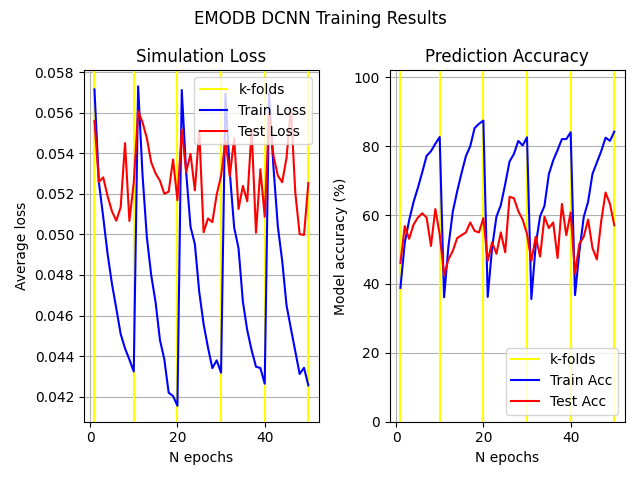
\includegraphics[scale = 0.6]{images_results/EMODB-FinalResults/EMODB_TrainResults_30-05__19-27.png}
        \caption{EMODB - K-Fold Test: ResNet18}
        \label{pilot_r18_fig}
\end{figure}
\subsubsection{ResNet34 Testing}
Next the more complex model, ResNet34 was plotted. This model was considered as a mid-point between the complexity of ResNet50 and the simplicity and potential for lower variance of ResNet18. Results are highlighted in \ref{pilot_r34_fig}, detailing worse performance than ResNet18. The average highest accuracy over each of the 10 epoch folds was \textbf{60.53\%}. While this difference is not dramatic, it definitely points to the fact that greater generalization improves the overall performance of the model for this dataset. 
\begin{figure}[ht]
        \centering
        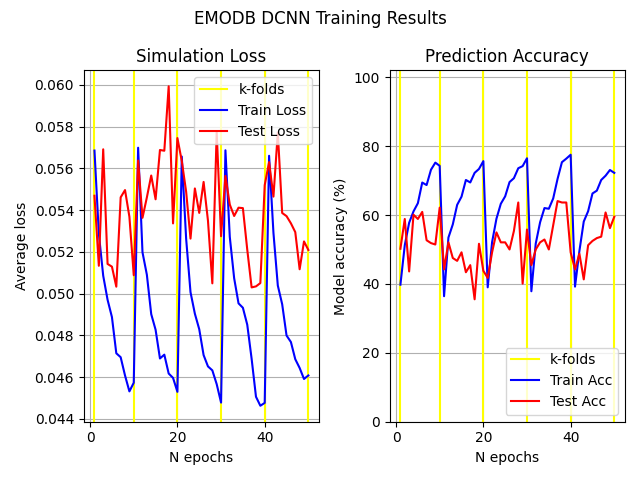
\includegraphics[scale = 0.6]{images_results/EMODB-FinalResults/EMODB_TrainResults_30-05__19-39.png}
        \caption{EMODB - K-Fold Test: ResNet34}
        \label{pilot_r34_fig}
\end{figure}
\subsubsection{ResNet50 Testing}
ResNet50 was then tested using a k-fold cross validation approach. As previous, the model parameters were held constant allowing independent grading of the model. Interestingly, the performance was greater than the ResNet34 model. Although not significantly enough to grade it as a better outright choice. This approach obtained an average highest accuracy of \textbf{61.03\%} over each of the folds. Demonstrating this, one may observe figure \ref{pilot_r50_fig}.
\begin{figure}[ht]
        \centering
        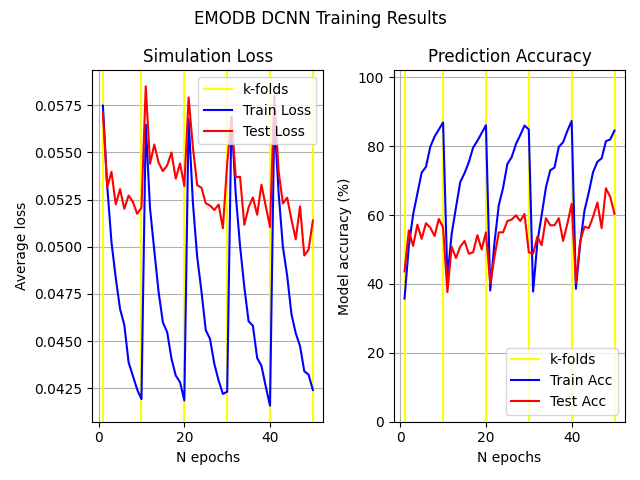
\includegraphics[scale = 0.6]{images_results/EMODB-FinalResults/EMODB_TrainResults_30-05__19-58.png}
        \caption{EMODB - K-Fold Test: ResNet50}
        \label{pilot_r50_fig}
\end{figure}

\subsection{Model Structure and Results}
The final results for the EMODB dataset were attained through use of the ResNet18 model with the additional output layers specified previously in this chapter. Model parameters are listed below. 
\begin{itemize}
    \item base model = ResNet18
    \itemsep0em
    \item epochs = 10
    \itemsep0em
    \item mini batch size = 32
    \itemsep0em
    \item k folds = 5
    \itemsep0em
    \item $lr = 1e^{-4}$
    \itemsep0em
    \item $\lambda$ = $1e^{-5}$
    \itemsep0em
    \item CyTex overlap = $0\%$
    \itemsep0em
    \item no learning rate scheduler implemented
    \itemsep0em
    \item data augmentation (training) = normalization
    \itemsep0em
\end{itemize}
Data augmentation strategies were removed from this approach to create more similar training and test data. This improved the score and while it may lead to overtraining, this should not influence generalization heavily over a small number of epochs. The approach was to reduce model bias rapidly as the pilot testing showed that numerous generalization strategies did not improve the results. A pseudo early stopping criteria was applied in which the parameters of the model with the net highest test accuracy were saved. This preserves a high test accuracy and will minimise the potential for overtraining. The highest accuracy obtained throughout the cross validation process was \textbf{72.7\%} test accuracy. The average test accuracy across each of the folds was \textbf{70.27\%}. The results over each fold are observed in figure \ref{emodb_final_results}.
\begin{figure}[ht]
        \centering
        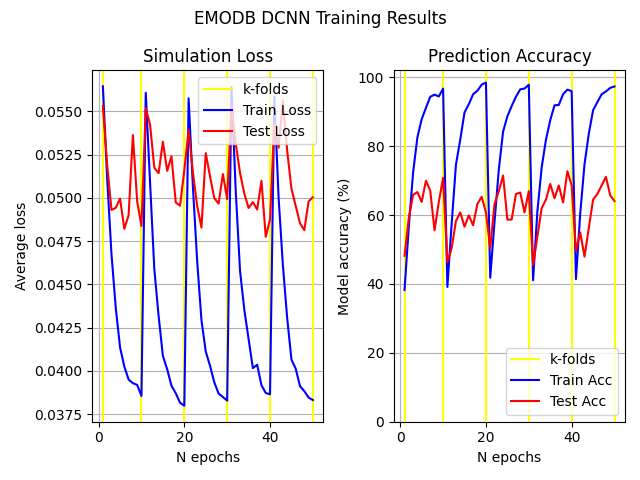
\includegraphics[scale = 0.6]{images_results/EMODB-FinalResults/EMODB_Results_31-05__15-50.png}
        \caption{EMODB - Final Training Results}
        \label{emodb_final_results}
\end{figure}

% SECTION:
% ================================================
\section{RAVDESS Simulations}
This section is significantly shorter than the EMODB results as that database formed the primary set for experimentation and grading model performance. Brief discussions of pilot testing and alterations to the data are included. However, only the final results of the RAVDESS dataset classification are inserted. Other test results can be found on the GitHub repository for this study \cite{Blake_ELEC4840B-Repo}. 

\subsection{Pilot Testing and Alterations}
As mentioned earlier, the results of the EMODB pilot test were largely applicable to the RAVDESS dataset as well. Experiments were conducted, however, roughly the same conclusions were made. The same base model and approximate parameters were identified to give the highest test accuracy. These remained largely unchanged from the previous cases and are detailed in the cross validation  discussion of results on the RAVDESS dataset. The primary difference is the larger number of epochs used due to the greater database size. The RAVDESS dataset took longer to train on in terms of both time and convergence to a solution.

\subsection{Dataset Reduction of Scope}
The RAVDESS dataset possessed more emotions than the EMODB dataset, (8 emotions as compared to 7). As such, the classification was slightly more difficult in this particular case. In attempts to further improve the test accuracy of this method, the number of emotional states for classification was reduced. The reduction of emotional states has been shown to increase a model's prediction accuracy, reducing the number of output classes \cite{zhou2016deep}. In the case of the RAVDESS dataset, the emotions Calm and Surprised exhibit similar characteristics to other emotions present in the dataset. For instance, surprise, prosodically, has features which overlap with fear and happiness given the context of the situation. Calm can also be closely related to a neutral emotion. In terms of the CyTex images generated for both of these emotions, it may be the case that they do not separate themselves enough, saliently, from other emotions in the dataset. Both of these emotions also had no direct equivalent in the EMODB dataset. For these reasons the dataset was truncated to exclude surprised and calm emotional classes for comparison. Results prior to, and after, emotional state truncation are provided in the successive section.

\subsection{Model Structure and Results}
Parameters for RAVDESS simulation were unchanged apart from the duration of simulation and exposure to the training sets. All notable parameters and formats are provided in the ensuing list. A ResNet18 model was once again utilised to reduce complexity of the model. A ResNet50 architecture was also trialled, however, inferior results were obtained.
\begin{itemize}
    \item base model = ResNet18
    \itemsep0em
    \item epochs = 14
    \itemsep0em
    \item mini batch size = 32
    \itemsep0em
    \item k folds = 5
    \itemsep0em
    \item $lr = 1e^{-4}$
    \itemsep0em
    \item $\lambda$ = $1e^{-5}$
    \itemsep0em
    \item CyTex overlap = $0\%$
    \itemsep0em
    \item no learning rate scheduler implemented
    \itemsep0em
    \item data augmentation (training) = normalization
    \itemsep0em
\end{itemize}
For the entire RAVDESS dataset an average test accuracy, across 5 folds, of \textbf{50.72\%} was recorded. As expected, reducing the number of output classes yielded a higher average test accuracy of \textbf{56.87\%}. These metrics relate to the results presented in figures \ref{ravdess_final_results} and \ref{ravdess_trunc_results}, respectively. The differences in accuracy between this dataset and the EMODB dataset are discussed in the following section. While these results are not as favourable as previous recordings, they do not form the primary judgement over the models performance. Further, the original CyTex study did not include exploration of this dataset, so the comparison to CyTex's previous performances cannot be made. One point of interest is that the initial accuracy of each fold is considerably lower than that of figure \ref{emodb_final_results}. This suggests that the base model and initial weights have more trouble describing and classifying the data in this set. In future trials, a slower converging extended epoch simulation should be conducted. This method would more intimately explore the characteristics and could benefit from the increased size of the RAVDESS dataset. While approaches similar to this were attempted, no promising results were gathered.
\begin{figure}[ht]
        \centering
        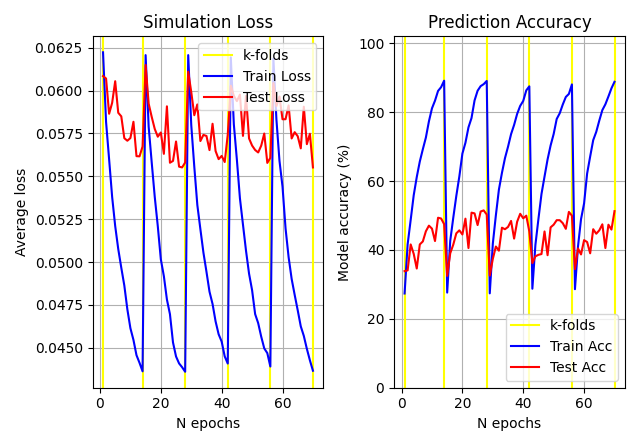
\includegraphics[scale = 0.6]{images_results/RAVDESS-FinalResults/RAVDESS_Results_31-05__19-18.png}
        \caption{RAVDESS - Final Training Results}
        \label{ravdess_final_results}
\end{figure}
\begin{figure}[ht]
        \centering
        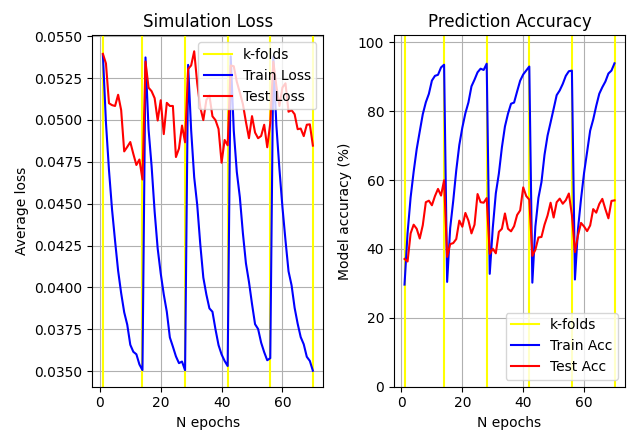
\includegraphics[scale = 0.6]{images_results/RAVDESS-FinalResults/RAVDESS_Results_01-06__12-17.png}
        \caption{RAVDESS - Truncated Data Results}
        \label{ravdess_trunc_results}
\end{figure}

% SECTION:
% ================================================
% PROBABLY NOT NECESSARY
% \section{Advanced Simulations}
% \textbf{*** Only add this section if given extension to alter CyTex images and further improve results. Also could include MEL Spectrogram results here.}


% SECTION:
% ================================================
\section{Discussion of Results}
This section discusses the results obtained for the two datasets considered in this study. The result achieved for the EMODB case is of a relatively high standard and is compared to validation/test results obtained by Zhao et al. \cite{ZHAO2019}. A discussion of the experimental design for achieving these results is covered. This includes information on how these results should be interpreted and whether or not they are directly comparable to other benchmark methods (including the foundational CyTex paper on which this work is based).  Concluding this section, suggestions for future experiments are put fourth with hopes of improving these results in further trials. The key results which will be referenced throughout this section pertain to table \ref{CytexResults_table}.
\begin{table}[ht]
    \centering
    \begin{tabular}{|l|c|c|}
    \hline
    Database & \multicolumn{1}{l|}{Highest Test Accuracy} & \multicolumn{1}{l|}{Average Fold Test Accuracy} \\ \hline
    \textbf{EMODB}             & 72.7\%  & 70.27\% \\ \hline
    \textbf{RAVDESS}           & 51.48\% & 50.72\% \\ \hline
    \textbf{Truncated RAVDESS} & 59.94\% & 56.87\% \\ \hline
    \end{tabular}
    \caption{Summary of CyTex Results}
    \label{CytexResults_table}
\end{table}

\subsection{Interpreting \& Comparing Results}
The main metrics used to gauge the performance of a model on a particular dataset in this report is the average test accuracy over five folds. This metric is often used in SER  literature due to the small  size of many widely used datasets. Another common measure is the average accuracy found over each of the emotional classes. This measure was not used at it does not accurately enough imply how a model may generalize. However, it does provide greater insight into particular classes or features that the model may have trouble classifying. In future this metric should also be included for a greater breadth of comparison.\\ \\
When comparing these results to contemporary benchmarks, we must first find suitable points of comparison. For the results on the EMODB dataset, the highest accuracy achieved rivals the validation accuracy observed in figure \ref{zhao2019_train_fig} \cite{ZHAO2019}. As this is considered a state  of the art method, our models achieves a good result in the training and validation phase. However, the average accuracies recorded over classes is likely significantly higher than this study of the CyTex methodology.\\ \\
The original results of Bakhshi et al. using the CyTex transform may be noted as significantly more accurate \cite{CyTexRef}. However, it is important to note the differences in experimental approach. A much more complicated base model of ResNet152 was utilised for their approach. More advanced computing resources were also available, which can have a direct impact on the accuracy of an assessed system. It is also likely that the quality and structure of CyTex images generated are noticeably different. The exact same process of image generation was not used, so it is likely that the parameters used in this study's approach are not as optimal as those used in the foundational study. This is also evidenced by the large gap between training and test accuracy in all figures detailing the training results of this thesis. A large training accuracy highlights the fact that the model is successful at identifying patterns in the training data. No difficulties exist that prevent the model from adequately learning. This points to the source of mismatch in accuracy metrics resulting from the CyTex images themselves. Despite the model learning, the images are not expressive or salient enough to yield more impressive results on validation sets. Potential improvements to the underlying CyTex images are discussed later.\\ \\
As far as the results evaluated on the RAVDESS dataset, significantly more work need be done to produce a noteworthy result. The TIM-Net model, currently holding one of the highest performance metrics for this dataset, is dramatically more accurate that the method detailed in this paper. TIM-Net achieves a UAR score of $91.93\%$ on this dataset \cite{ye2023temporal}. This approach employs 10-fold cross validation, and while it is not directly analogous to the metrics of table \ref{CytexResults_table}, it clearly details a need to improve this strategy's results.


\subsection{Improving Results in Further Experiments}
A number of strategies for improving the results are provided below. It is predicted that the greatest positive improvement of results would be seen by modification of the generated CyTex images used for training and evaluation. Methods for improving the validity and comparability of results are also discussed.
\subsubsection{CyTex Parameter Tuning}
As was noted, it is likely that the generated CyTex images are the source of less than optimal accuracy in each of the test settings. By further tuning parameters used to generate these images the quality of the transform should increase. It is important to note that these parameters may need to be tuned on a per dataset basis.\\ \\
The maximum frequency threshold ($\mathbf{f_{max}}$) able to be extracted by the librosa piptrack method should be stepped by intervals of $100Hz$. For experiments conducted in this work, a maximum of $400Hz$ was used as this should include the standard operating frequency of human speech. However, two potential scenarios could be affecting the resultant images. The first scenario is that the maximum threshold is too large and too much frequency data is included. This means that information that is not useful for the classification of emotional speech is making its way into the CyTex images. The other case is that the maximum threshold is too low and there exists data samples which exhibit frequencies larger than the maximum threshold. If this is the case, the piptrack method may be truncating important information that could inform the basis of classification.\\ \\
Framing can produce differing results as well. While $10ms$ is a common choice, this value may not be optimal for the RAVDESS dataset. Some literature uses values somewhat larger than this interval, which could change the performance of a model. Values significantly larger should not be used, however. This would result in speech frames that are no longer able to be considered stationary and the granularity of fundamental frequencies extracted would be too coarse. Varying this frame length between $10ms$ and $40ms$ may produce some difference to the observed results, particularly for the RAVDESS database. It has been found, experimentally, that $10ms$ is a suitable measure for the EMODB database experiments.\\ \\
Finally, the additional dimensions of encoding the RGB images could be substituted for different kinds of information. Horizontal and vertical gradients were used in this application, but this information may not be optimal. A wealth of other encoding schemes could be used, including previously discussed strategies like Laplace Transform information.

\subsubsection{MEL Spectrogram Comparison}
In order to better determine whether the model needs improvement and to give a better baseline for model performance, MEL-Spectrograms should be generated for each of the samples in a given dataset. The model can then be trained and evaluated on this set of image data. We expect the performance of a properly employed CyTex method to be greater than that of a MEL spectrogram approach. If this is not the case, we can infer that our CyTex images need be further improved to better represent the dataset. If the MEL-Spectrogram trained model also performs poorly, it is inferred that the model is a poor candidate for exhibiting exemplary results.

\subsubsection{Alternate Performance Metrics}
During this thesis, only training and validation sets were used. This is why the terms test and validation have been used interchangeably in places. The decision to do so was to recreate the experimental conditions from the original CyTex study conducted by Bakhshi et al. The small size of a dataset like the EMODB also necessitates this as splitting this set into 3 subsets (training and independent test and validation sets) can compromise the validity of results. In this case, either the test and validation sets will be too small to gain meaningful information about generalization. Or, the training set will be too small to sufficiently learn the model. That being said, in future the use of independent test and validation sets would help obtain results that are more closely comparable to other studies in the literature.

\subsubsection{Data Augmentation Injection}
Thanapol et al. suggest improved generalization using a novel approach to data augmentation \cite{Thanapol2020}. In this study, CNN models are initially trained on non-augmented data samples, similarly to the approach taken in this thesis. This encourages an initial fast convergence to a solution. However, after 30 epochs the training data is inject with data augmentations. This means that after a model has learned the more basic features to broadly classify input data, it then gains a better capacity to generalise, minimising overfitting. An approach like this would be interesting to study and may improve performance metrics.

